\hypertarget{reduce-reuse-recycle}{%
\subsection{Reduce, reuse, recycle}\label{reduce-reuse-recycle}}

\hypertarget{motivation}{%
\subsubsection{Motivation}\label{motivation}}

This pattern can guide project participants in identifying and managing
available resources.

\hypertarget{context}{%
\subsubsection{Context}\label{context}}

In a peer production context, you are simultaneously ``making stuff''
and building on the work of others.

\hypertarget{forces}{%
\subsubsection{Forces}\label{forces}}

\begin{quote}

\includegraphics{images/derivative.png} \textbf{Derivative}: you don't
have to do everything yourself!\\

\includegraphics{images/sensemaking.png} \textbf{Sensemaking}: resources
are useful only when you can make sense of them.\\

\includegraphics{images/sharing.png} \textbf{Sharing}: your
understanding gains robustness when you share with others.
\end{quote}

\hypertarget{problem}{%
\subsubsection{Problem}\label{problem}}

Many projects die because the cost of
{{\href{http://c2.com/cgi/wiki?ReinventingTheWheel}{Reinventing the
Wheel}}} {[}c2{]} is too high. However, this is just one possible
symptom of overfocus on a few priorities. Concerns may also arise if the
project's output is not actually used by anyone.

\hypertarget{solution}{%
\subsubsection{Solution}\label{solution}}

``Steal like an artist,'' and make it possible for other people to build
on your work too. In the Peeragogy project, we have used off-the-shelf
and hosted software suited to the task at hand (including: Drupal,
Google+, Google Hangouts, Google Docs, Wordpress, pandoc, Github,
ShareLaTeX). Early on we agreed to release our \emph{Peeragogy Handbook}
under the terms of the Creative Commons Public Domain Dedication (CC0),
the legal instrument that grants the greatest possible leeway to
downstream users.\footnote{\url{https://creativecommons.org/publicdomain/zero/1.0/}}
This has allowed us and others to repurpose and improve its contents in
other settings, including the current paper. Follow the steps indicated
by the keywords in the pattern's title:

\begin{itemize}
\tightlist
\item
  \emph{Reduce} the panoply of interesting interrelated ideas and
  methods to a functional core (e.g.~writing a book).
\item
  \emph{Reuse} resources relevant to this aim, factoring in ``things I
  was going to have to do anyway'' from everyone involved.
\item
  \emph{Recycle} what you've created in new connections and
  relationships.
\end{itemize}

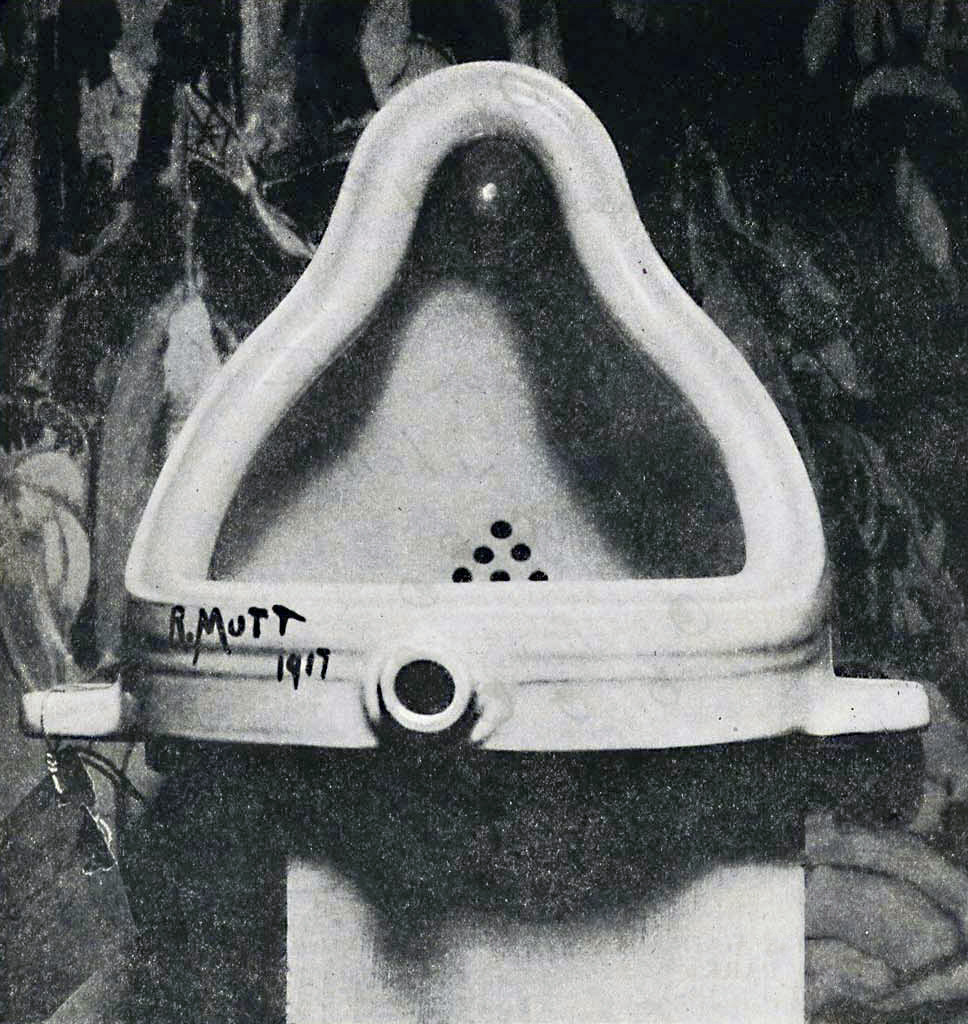
\includegraphics{images/Duchamp_Fountaine.jpg}\\
\emph{A paradigmatic example of found-art. ``Fountain by R. Mutt,
Photograph by Alfred Stieglitz, THE EXHIBIT REFUSED BY THE
INDEPENDENTS''.}

\hypertarget{rationale}{%
\subsubsection{Rationale}\label{rationale}}

Clearly we are not the first people to notice the problems with
wheel-reinvention, including ``missing opportunities, repeating common
mistakes, and working harder than we need to.''\footnote{\url{https://blog.wikimedia.org/2013/11/19/learning-patterns-new-way-share-important-lessons/}}
As a guest in one of our hangouts, Willow Brugh, of Geeks without Bounds
and the MIT Media Lab, remarked that \emph{people often think that they
need to build a community, and so fail to recognize that they are
already part of a community.}\footnote{\url{https://www.youtube.com/watch?v=NpyQfYVKfBI}}
converted our old pattern catalog from the \emph{Peeragogy Handbook}
into this paper, sharing it with a new community and gaining new
perspectives; could we do something similar again?

\hypertarget{resolution}{%
\subsubsection{Resolution}\label{resolution}}

Reweaving old material into \textbf{derivative} designs and new material
into existing frameworks, we build deeper understanding, and carry out
collective \textbf{sensemaking}. The project's {{Roadmap}} develops by
making sense of existing resources -- including our worries and
concerns. Often we only know what these are when we attempt to
\textbf{share} them. Drawing on a wide range of resources boosts our
collective {{Carrying capacity}}.

\hypertarget{example-1}{%
\subsubsection{Example 1}\label{example-1}}

Contributors are encouraged to recycle existing works that are
compatible with the Wikimedia-wide Creative Commons
Attribution-ShareAlike (CC-By-SA) license.\footnote{\url{https://creativecommons.org/weblog/entry/15411/}}
Some sub-projects have been created purely to help repurpose other
existing works in this way.\footnote{\url{https://en.wikipedia.org/wiki/Wikipedia:WikiProject_Mathematics/PlanetMath_Exchange}}
On the downstream side, DBPedia is an important resource for the
semantic web, built by collating data from Wikipedia's
``infoboxes.''\footnote{\url{http://wiki.dbpedia.org/}} themselves
increasingly being populated automatically using information from
WikiData.\footnote{\url{https://www.wikidata.org/wiki/Wikidata:Main_Page}}
able to develop tools that reuse Wikipedia content in other ways
{{[}1,2{]}}, However, these research projects do not always result in a
tool that is accessible to day-to-day users.

\hypertarget{example-2}{%
\subsubsection{Example 2}\label{example-2}}

The knowledge resources and collaboration tools currently available
online are what make a low-cost, high-quality, formally-accredited
future university conceivable. However, the available resources are not
always as organized as they would need to be for educative purposes, so
peeragogues can usefully put effort into {{Reduce, reuse, recycle}}'ing
available resources into a functioning university Library.

\hypertarget{whats-next-in-the-peeragogy-project}{%
\subsubsection{What's Next in the Peeragogy
Project}\label{whats-next-in-the-peeragogy-project}}

Are there other educational resources and peeragogical case studies that
we could fold into our work? Can we recycle material from the
\emph{Peeragogy Handbook} into a format that is easier to understand and
apply?

\hypertarget{references}{%
\subsubsection{References}\label{references}}

\begin{enumerate}
\def\labelenumi{\arabic{enumi}.}
\item
  Silvan Reinhold. 2006. WikiTrails: Augmenting wiki structure for
  collaborative, interdisciplinary learning. \emph{Proceedings of the
  2006 International Symposium on Wikis}, ACM, 47--58.
\item
  Nathalie Henry Riche, Bongshin Lee, and Fanny Chevalier. 2010. IChase:
  Supporting exploration and awareness of editing activities on
  Wikipedia. \emph{Proceedings of the International Conference on
  Advanced Visual Interfaces}, ACM, 59--66.
\end{enumerate}

\begin{center}\rule{0.5\linewidth}{0.5pt}\end{center}
